\chapter{Design}
\label{chap:design}

Design by mohl být definován jako aktivita, jejíž úkol je přenést nápad, představu nebo myšlenku něčeho užitečného do zpracovatelné podoby, ať už se jedná o auto, budovu, službu nebo proces. Je to množina činností, která má za úkol pomoct lidem v orientaci a učinit jejich život jednodušší. Design je všudypřítomný, ať už se nacházíme uvnitř budovy, na autobusovém nástupišti nebo procházíme Internetové stránky -- může to být model auta, interiér budovy nebo informační systém; představuje způsob jak věci vypadají, jak fungují a jak moc pozornosti přitahují nebo nepřitahují. Existují samozřejmě případy, kdy je nežádoucí, aby design přitahoval příliš mnoho pozornosti. Úkolem designera je tedy vžít se do role uživatele, do jeho chování a potřeb. Pouze designeři mohou proměnit koncept v něco žádoucího, hodnotného a komerčně úspěšného.

Ve 2. polovině 20. století se zrodil zcela nový obor anglicky nazvaný \textit{computer science}. Tento obor označujeme jako informatika. Informatika má zásadní vliv na design a to nejen na samotný proces tvorby, díky informačním technologiím vznikly zcela nové oblasti designu. Každá aplikace, služba nebo webová stránka potřebuje rozhraní, které bude sloužit jako vrstva komunikující s uživateli. Při vzniku prvních operačních systémů byla snaha vývojářů a designerů unifikovat grafické uživatelské rozhraní. Tato unifikace měla za úkol poskytnout uživatelům intuitivní prostředí a tím zredukovat nutnost porozumět všem variacím uživatelských rozhraní grafických aplikací. S rozšířením Internetu se toto úsilí přenáší především na designera a společnost je tak vystavena daleko většímu množství nových grafických rozhraní a technologií. Tento trend je zodpovědný za vznik mnoha nových pojmů a konvencí.

Mezi designery se v posledních letech rozšířilo několik nových termínů, které mají za úkol jednoznačně rozlišit jednotlivé činnosti a profily webdesignu. Podstatou těchto pojmů je zároveň usnadnění komunikace mezi designery, mezi ty nejpodstatnější patří --

\begin{itemize}
    \item Použitelnost (Usability)
    \item UI (User Interface)
    \item UX (User eXperience)
\end{itemize}

Tyto pojmy se navzájem prolínají. Jedná se především o soubor zásad a doporučení pro úspěšné dokončení tvorby uživatelského rozhraní.

\section{Použitelnost}
\label{sec:usability}

Použitelnost je soulad užitečnosti a jednoduchosti použití. Produkt (aplikace nebo zařízení) je použitelný pokud --

\begin{itemize}
    \item je pro uživatele užitečný a vyhovuje jeho potřebám
    \item je jednoduché naučit se produkt používat
    \item je efektivní produkt používat -- zabere málo času vykonat nějaký úkol
    \item je produkt málo náchylný na chyby
\end{itemize}

Dobře použitelný produkt musí do jisté míry splňovat všechny tyto body. Existuje mnoho produktů, které jsou natolik složité, že většinu uživatelů odradí od normálního používání (pokud mají možnost volby). Často se přitom jedná o vysoce užitečné a produktivní aplikace -- typickým příkladem jsou informační systémy, které obsahují ohromné množství dat a nástrojů se kterými musí uživatelé manipulovat.

\begin{figure}[htbp]
    \centering
    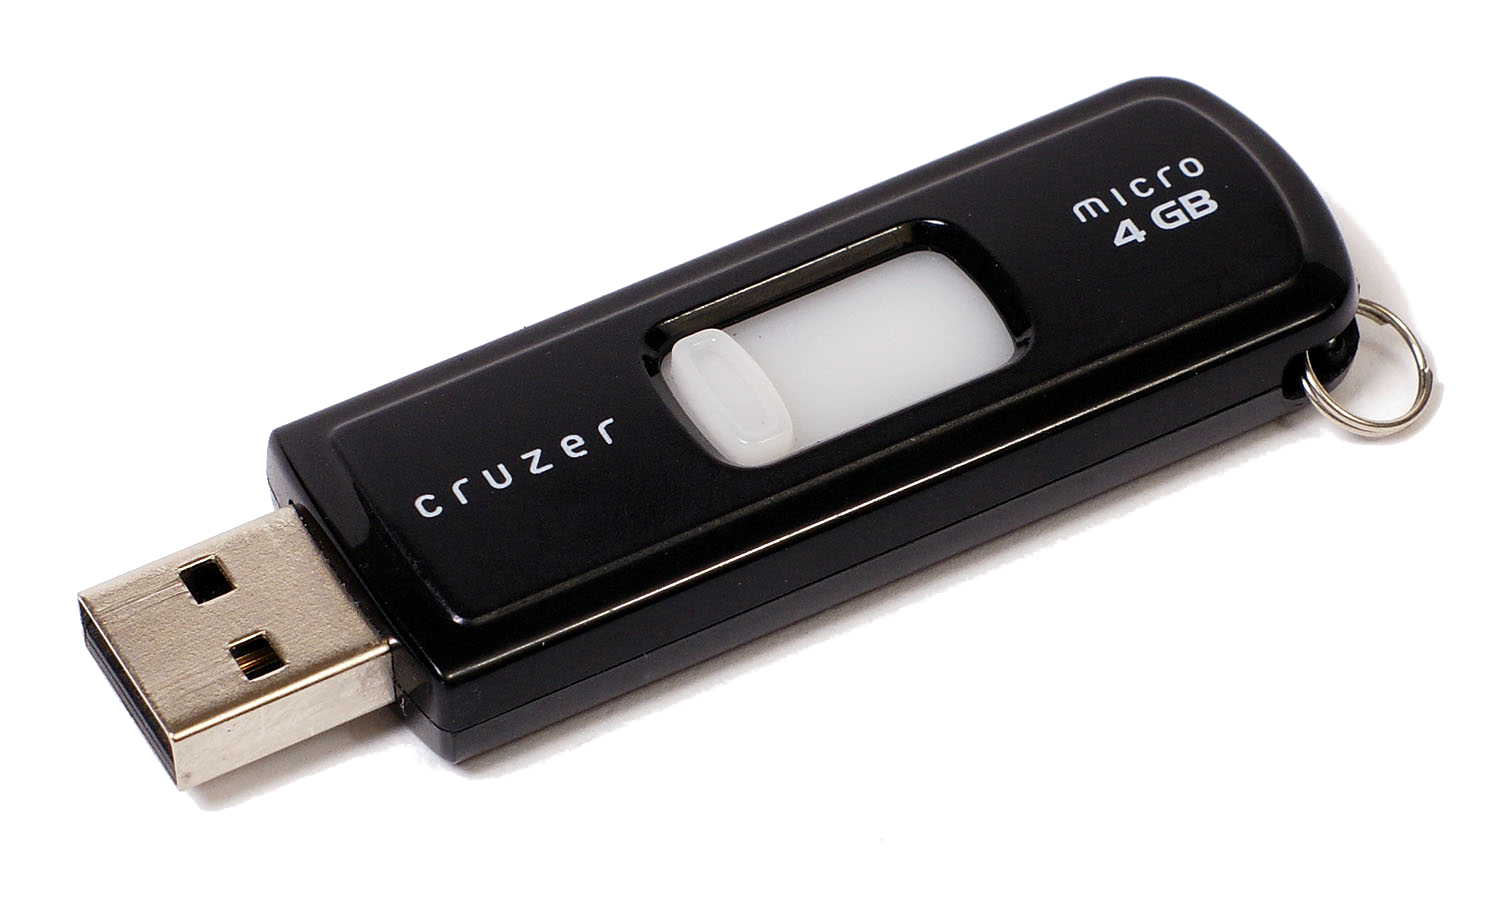
\includegraphics[width=11cm]{images/usb-fail.png}
    \caption{Špatná použitelnost USB standardu -- kterou stranou se připojuje zařízení k počítači?}
\end{figure}

Mezi některé typické příklady špatné použitelnosti webových aplikací patří například absence vyhledávače, nutnost registrace pro zobrazení většiny obsahu nebo dlouhé registrační formuláře a nečitelná CAPTCHA. Jednou z nejdůležitějších vlastností dobře použitelných aplikací je správná typografie (viz \ref{sec:typografie}).

\section{UI design}
\label{sec:uidesign}

UI design zahrnuje práci designerů, kteří vytvářejí hmatatelné prvky se kterými uživatele manipulují. UI designeři se soustředí na vizuální podobu a použitelnost produktů a služeb. Použitelnost je tedy nutnou součástí kvalitních uživatelských rozhraní.

Uživatelské rozhraní webových aplikací prošlo v posledních letech zásadním vývojem -- za tento vývoj je zodpovědná především rozšířenost webových technologií (HTML, CSS a JavaScript) a s tím související popularita majoritních webových prohlížečů. Ještě nedávno patřil mezi nejpopulárnější prohlížeče Internet Explorer, který má dodnes nejhorší podporu moderních webových technologií.

\section{UX design}
\label{sec:uxdesign}

UI design je část produktu, se kterou přichází uživatel do kontaktu, když se na produkt podívá. UX design je pocit, jaký uživatel má, když produkt používá \cite{ui-vs-ux}. UI design je pouze částí UX designu, stejně jako použitelnost je součástí UI designu (viz obrázek \ref{fig:ux-ui-usability}).

\begin{figure}[htbp]
    \centering
    \includegraphics[width=10cm]{images/ux.pdf}
    \caption{Podíl UX, UI a použitelnosti v designu.}
    \label{fig:ux-ui-usability}
\end{figure}

Příklad některých prvků, které mají vliv na dobrý UX design \cite{understanding-ux-ui}.

\begin{itemize}
    \item \textbf{Obsah}. Kvalita obsahu, struktura textu obrázků a dalších typografických prvků.
    \item \textbf{Dostupnost pomoci}. Online chat, email technické podpory.
    \item \textbf{Výkon}. Rychlost stránek a dostupnost.
    \item \textbf{Diskuze}. Podpora diskuzí a hodnocení produktů.
    \item \textbf{Způsob platby}. Možnost internetové platby (platba kartou, PayPal apod.)
    \item \textbf{Reklama}. Výskyt reklam a jejich způsob zobrazení.
\end{itemize}

\section{Typografie}
\label{sec:typografie}

\begin{quote}
    \uv{Typografie je organizace písma v ploše} \cite{svalbach}
\end{quote}

\noindent
Typografie je ještě starší než samotný design, její počátky sahají do 15. století, kdy Johannes Gutenberg vynalezl knihtisk. Už tehdy si typografové uvědomovali její důležitost. Během nadcházejících století se typografie rozšířila do novin, informačních systémů nebo reklam. Popularita typografie měla za následek rozvoj mnoha rodin písma, které se používají i u dnešních displejů elektronických zařízení.

Webdesign je z 95\% typografie -- toto tvrzení vyplývá ze skutečnosti, že 95\% informací na internetu se nachází v písemné podobě \cite{typography}. Typografie je zásadním prvkem pro tvorbu webových aplikací, jedná se o primární způsob přenosu informací mezi aplikací a uživatelem. Tento fakt klade určité nároky na kvalitní uživatelská rozhraní, které vycházejí z knižní typografie.

\subsection{Volba čitelných fontů}

Pro nadpisy a podnadpisy je doporučené používat patkové písmo, naopak pro menší text bezpatkové. Displeje s nízkým PPI (počtem pixelů na palec) radikálně snižují čitelnost patkových fontů.

\subsection{Šířka odstavců}

Příliš dlouhé řádky textu snižují soustředěnost. Tento jev je dán nutností čtenáře získat představu o tom, kde řádek končí a kde nový začíná. Naopak krátké řádky nutí návštěvníka číst příliš přerušovaně. Délka odstavce by měla odpovídat přibližně 55--80 znakům na řádek.

\subsection{Velikost písma}

Minimální doporučovaná velikost písma je 16$px$, což je přibližně stejná velikost, jako velikost textu vytištěného v knize nebo v magazínu \cite{min-font-size}.

\subsection{Řádkování}

Podobně jako šířka odstavců i řádkování ovlivňuje nutnost koncentrace čtenáře. Minimální doporučené řádkování je 1.3$em$.

\subsection{Velikost okrajů}

Okraje oddělují důležitý obsahu od ostatních částí webu a dovolují čtenáři soustředit se na text. Doporučený poměr okrajů na webu je 2:3:4:3 (vrch \textbf{:} pravá strana \textbf{:} spodek \textbf{:} levá strana), velikost okrajů pak 2$em$ \textbf{:} 3$em$ \textbf{:} 4$em$ \textbf{:} 3$em$, kde 1$em$ je roven dvojnásobku velikosti fontu.

\subsection{Kontrast textu}

Kontrast má velký vliv na čitelnost, nízký kontrast zvyšuje únavu očí, naopak příliš vysoký kontrast působí dráždivě \cite{eye-strain}. Jedna z doporučených kombinací je tmavě šedý text na bílém pozadí.

\begin{figure}[htbp]
    \centering
    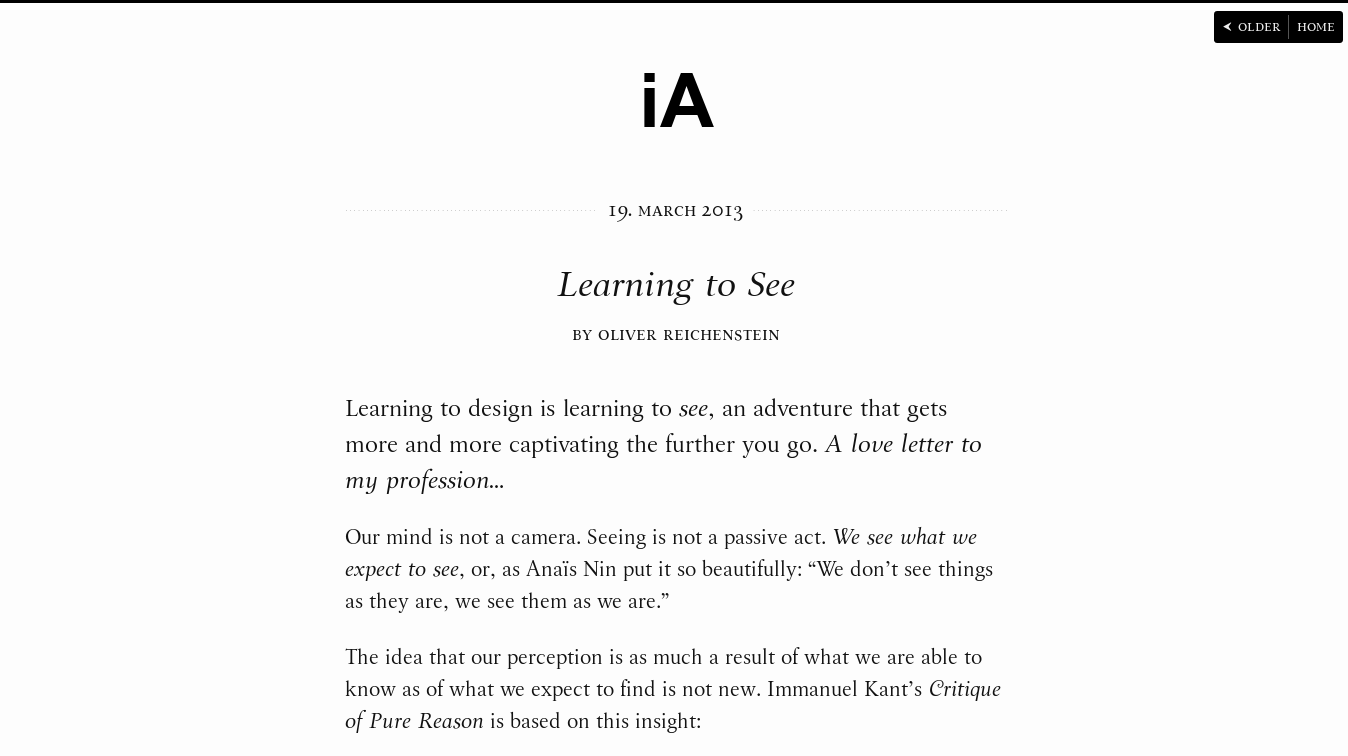
\includegraphics[width=11cm]{images/typography.png}
    \caption{Příklad webové stránky s výhradně typografickými prvky. Můžeme si všimnout, že autor použil na celé stránce pouze jednu rodinu písma. Zdroj: \url{http://informationarchitects.net/}.}
    \label{fig:web-typography}
\end{figure}
